\documentclass{beamer}
%
% Choose how your presentation looks.
%
% For more themes, color themes and font themes, see:
% http://deic.uab.es/~iblanes/beamer_gallery/index_by_theme.html
%
\mode<presentation>
{
  \usetheme{Darmstadt}      % or try Darmstadt, Madrid, Warsaw, ...
  \usecolortheme{orchid} % or try albatross, beaver, crane, ...
  \usefonttheme{professionalfonts}  % or try serif, structurebold, ...
  \setbeamertemplate{navigation symbols}{}
  \setbeamertemplate{caption}[numbered]
} 

\usepackage[english]{babel}
\usepackage[utf8x]{inputenc}
\usepackage{tikz}
\usetikzlibrary{arrows}

\usepackage{amsmath, amssymb, amsthm, amsfonts}
\centering

\newcommand{\C}{\mathbb{C}}
\newcommand{\N}{\mathbb{N}}
\newcommand{\Q}{\mathbb{Q}}
\newcommand{\R}{\mathbb{R}}
\newcommand{\Z}{\mathbb{Z}}
\newcommand{\Lra}{\Leftrightarrow}
\newcommand{\dsp}{\displaystyle}
\newcommand{\Xbar}{\overline{X}}
\newcommand{\abs}[1]{\big| #1 \big|}




\title[Ebola Dynamics]{Ebola Dynamics}
\author{Chelsea Sandridge, Colton Bryant, Kelsey Kalmbach, Paul Diaz, and Sean Lopp}
\institute{Colorado School of Mines}
\date{\today}

\begin{document}

\section{Introduction}

\begin{frame}
  \titlepage
\end{frame}

\begin{frame}{Outline}
   \tableofcontents
\end{frame}


\section{The Model}

\subsection{Model Assumptions}

% \begin{frame}{Model Assumptions}
% \begin{itemize}
% \item Infected individuals can move to three different compartments: Removed and infectious, removed and buried, removed and recovered. 
% \item Individuals who have died from the disease but who have not yet been buried can still infect susceptible individuals.
% \item Individuals who recover from the disease are no longer susceptible
% \item Once hospitalized, infected individuals can still infect others. However, those who die in the hospital are buried immediately, and thus cannot infect others once dead.
% \item Hospitals have unlimited space, but there is some delay in hospitalization.
% \end{itemize}


% \end{frame}

\subsection{Variable Definitions}

% \begin{frame}{Variable Definitions}
% \textbf{Populations:} \\
% \raggedright
% $S = $ Susceptible Population \\
% $E = $ Exposed Population (infected but not yet showing symptoms) \\
% $I = $ Infectious Population \\
% $H = $ Hospitalized Population \\
% $R_I = $ Removed and Infectious Population (dead but not yet buried) \\
% $R_B = $ Removed and Buried \\
% $R_R = $ Removed and Recovered \\
% \end{frame}

\subsection{State Diagram}

\begin{frame}{State Diagram}
\tikzstyle{line} = [draw, -latex']
\begin{figure}[ht!]
\begin{center}
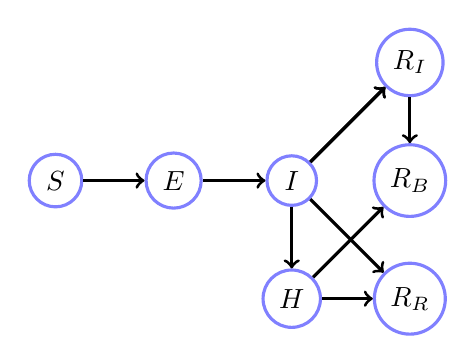
\begin{tikzpicture}[place/.style={circle,draw=blue!50,line width=0.4mm, fill=white},
   transition/.style={->,line width=0.4mm}, scale = 0.5]
\node[place] (s) at (-6, 0) {$S$};
\node[place] (e) at (-3, 0) {$E$};
\node[place] (i) at (0, 0) {$I$};
\node[place] (rb) at (3, 0) {$R_B$};
\node[place](ri) at (3, 3) {$R_I$};
\node[place](rr) at (3, -3) {$R_R$};
\node[place](h) at (0, -3) {$H$};

\path
    (s) edge[transition] node[auto]{} (e)
    (e) edge[transition] node[auto]{} (i)
    (i) edge[transition] node[auto]{} (ri)
    (ri) edge[transition] node[auto]{} (rb)
    (i) edge[transition] node[auto]{} (ri)
    (i) edge[transition] node[auto]{} (rr)
    (i) edge[transition] node[auto]{} (h)
    (h) edge[transition] node[auto]{} (rr)
    (h) edge[transition] node[auto]{} (rb)

;
            

\end{tikzpicture}
\caption{Illustration of mathematical model}
\label{tikz3CM}
\end{center}
\end{figure}


\end{frame}



\begin{frame}{Variable Definitions}
\textbf{Parameters:} 
\scriptsize
\begin{align*}
\alpha &= \text{population growth constant} \cite{WorldBank} \\
\beta_1 &= \text{transmission rate between infected and susceptible} \\
\beta_2	&= \text{transmission rate between removed and still infectious and susceptible} \\
\beta_3 &= \text{transmission rate between hospitalized and susceptible}\\
\delta &= \text{rate at which people move from exposed to infected}\ \cite{CDC2} \\
\gamma_1 &= (\text{average time with disease for unhospitalized individuals} )^{-1}\\
\gamma_2 &= (\text{average time with disease for hospitalized individuals} )^{-1}\\
\psi &= (\text{average time that people become hospitalized})^{-1}\\
\rho_1 &= 1.1\times \rho_2 = \text{the proportion of people who die of the disease who are not hospitalized}\ \cite{epic} \\
\rho_2   &= \text{the proportion of people who die of the disease who are hospitalized}\ \cite{epic} \\
\omega  &= (\text{time until one is buried})^{-1}
\end{align*}
\end{frame}

\subsection{The Model}

\begin{frame}{The Model}
\begin{align*} 
\frac{dS}{dt} &= \alpha S - \beta_1 S I -\beta_2 S R_I -\beta_3SH\\
\frac{dE}{dt} &=  \beta_1 S I +\beta_2 S R_I +\beta_3SH- \delta E \\
\frac{dI}{dt} &=  \delta E - \gamma_1 I-\psi I\\
\frac{dH}{dt} &= \psi I - \gamma_2 H \\ 
\frac{dR_I}{dt} &= \rho_1\gamma_1 I - \omega R_I \\
\frac{dR_B}{dt} &= \omega R_I+\rho_2\gamma_2 H \\ 
\frac{dR_R}{dt} &= (1-\rho_1)\gamma_1 I+(1-\rho_2)\gamma_2 H \\
\end{align*}

\end{frame}




\section{Simulations}

\subsection{Speed Test}
\begin{frame}{Speed Test}
\centering
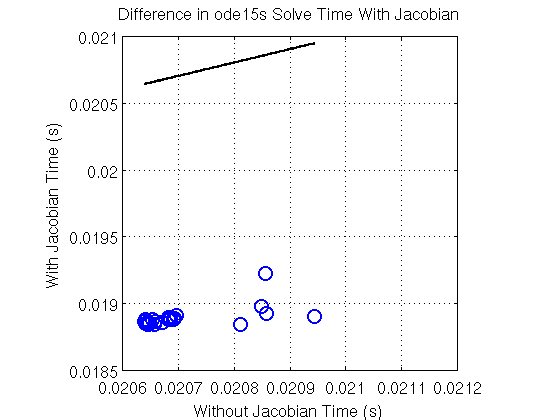
\includegraphics[scale=0.6]{jacnojac}
\end{frame}

\subsection{Accuracy Analysis}
\begin{frame}{Errors for varying tolerances} 
\centering
\begin{figure}[ht!]
\centering
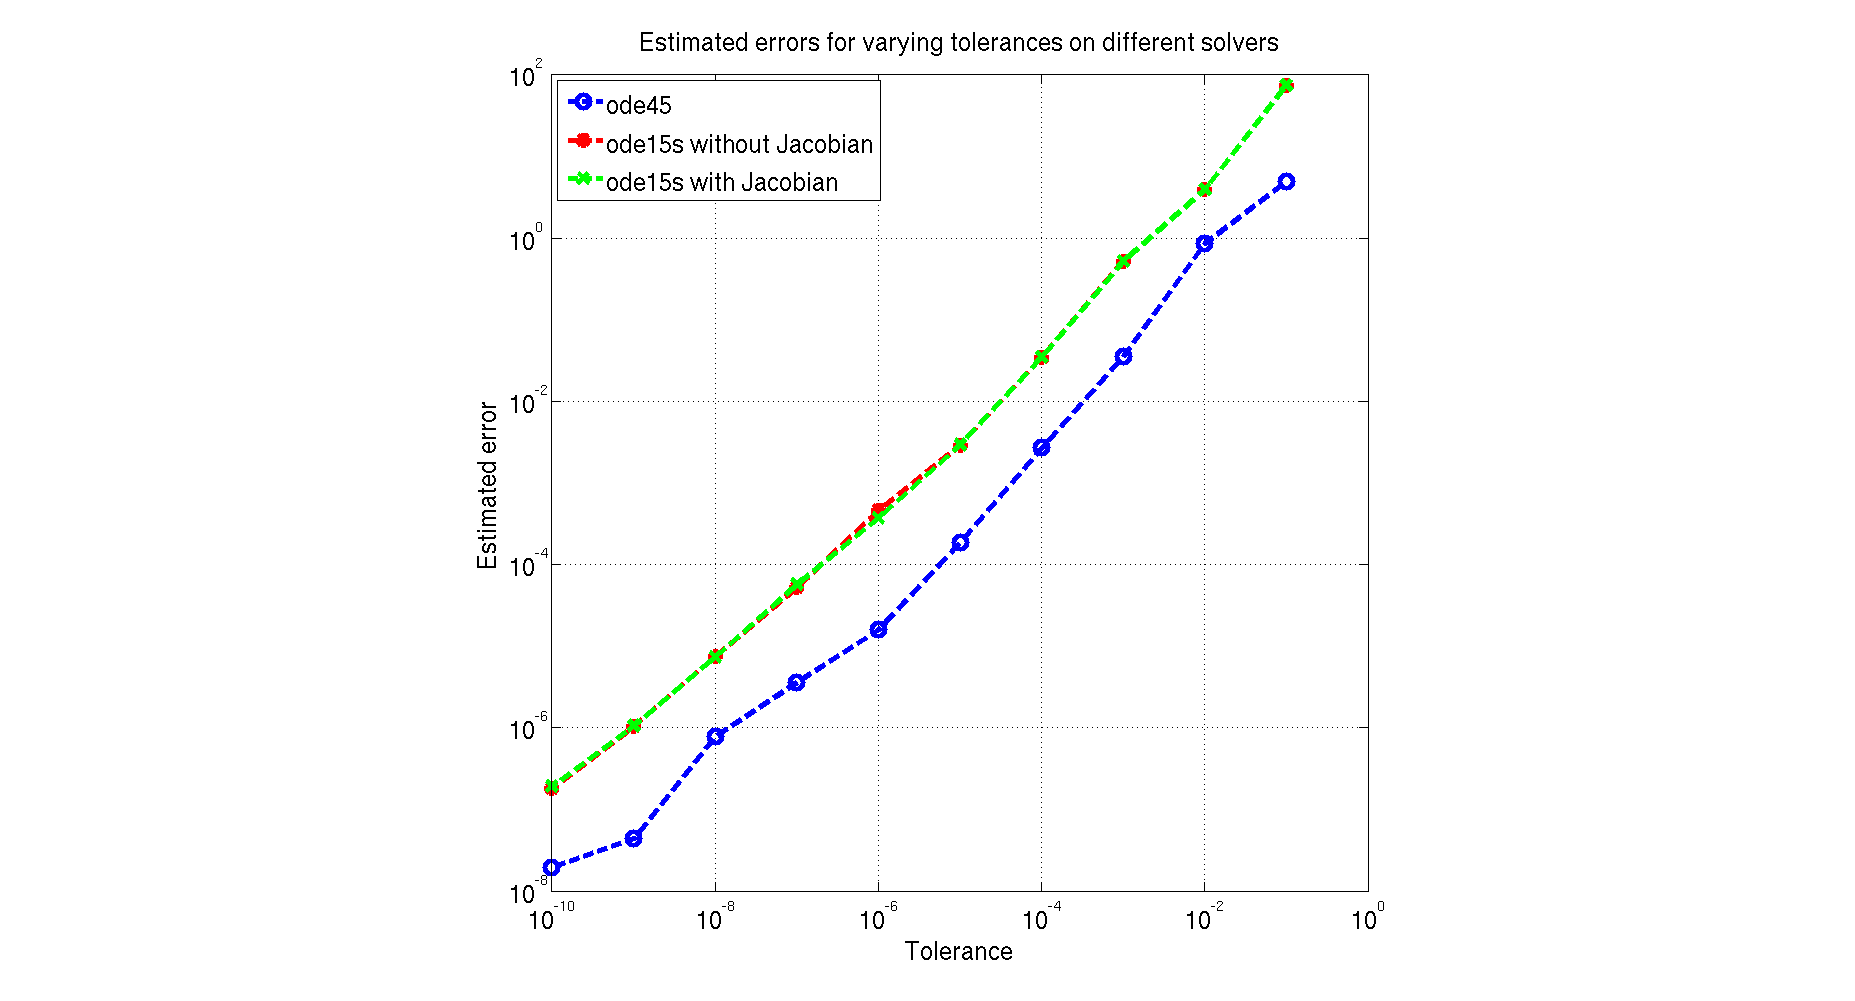
\includegraphics[scale=0.25]{errorvtol} 
\end{figure}
\end{frame}

\begin{frame}{Times to compute and resulting errors}
\centering
\begin{figure}[ht!]
\centering
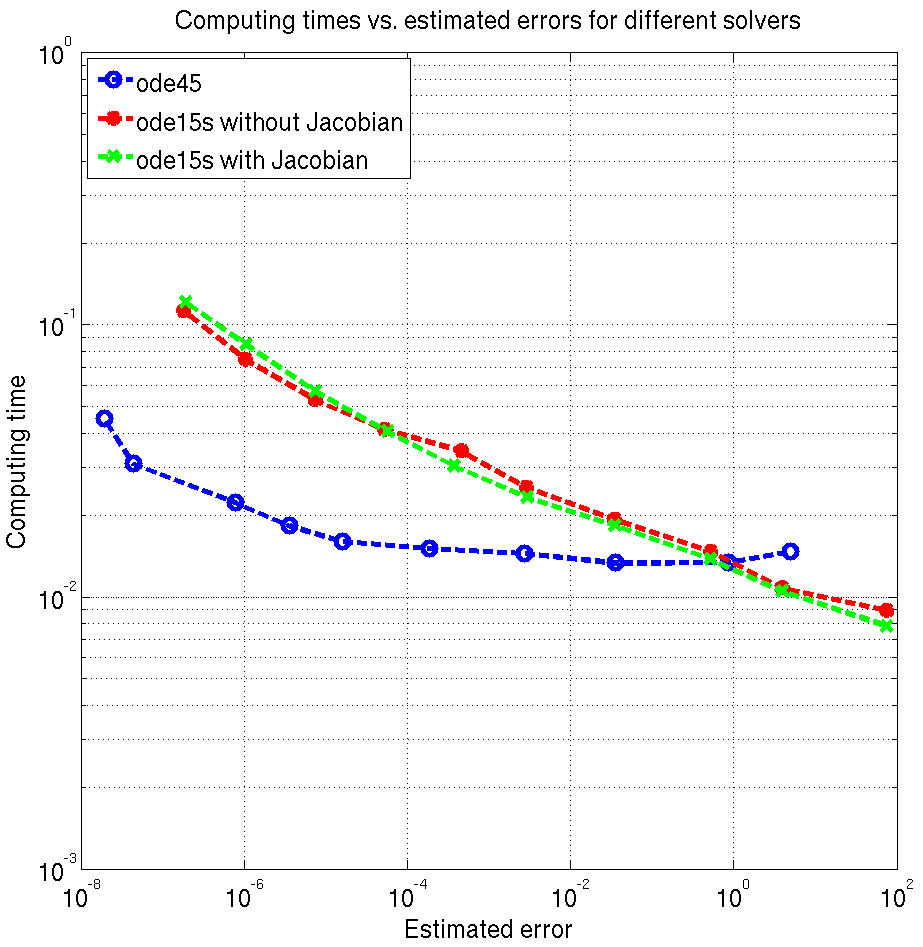
\includegraphics[scale=0.2]{timeverror} 
\end{figure}
\end{frame}

\subsection{Model Simulation}
\begin{frame}{Model Simulation}
\centering
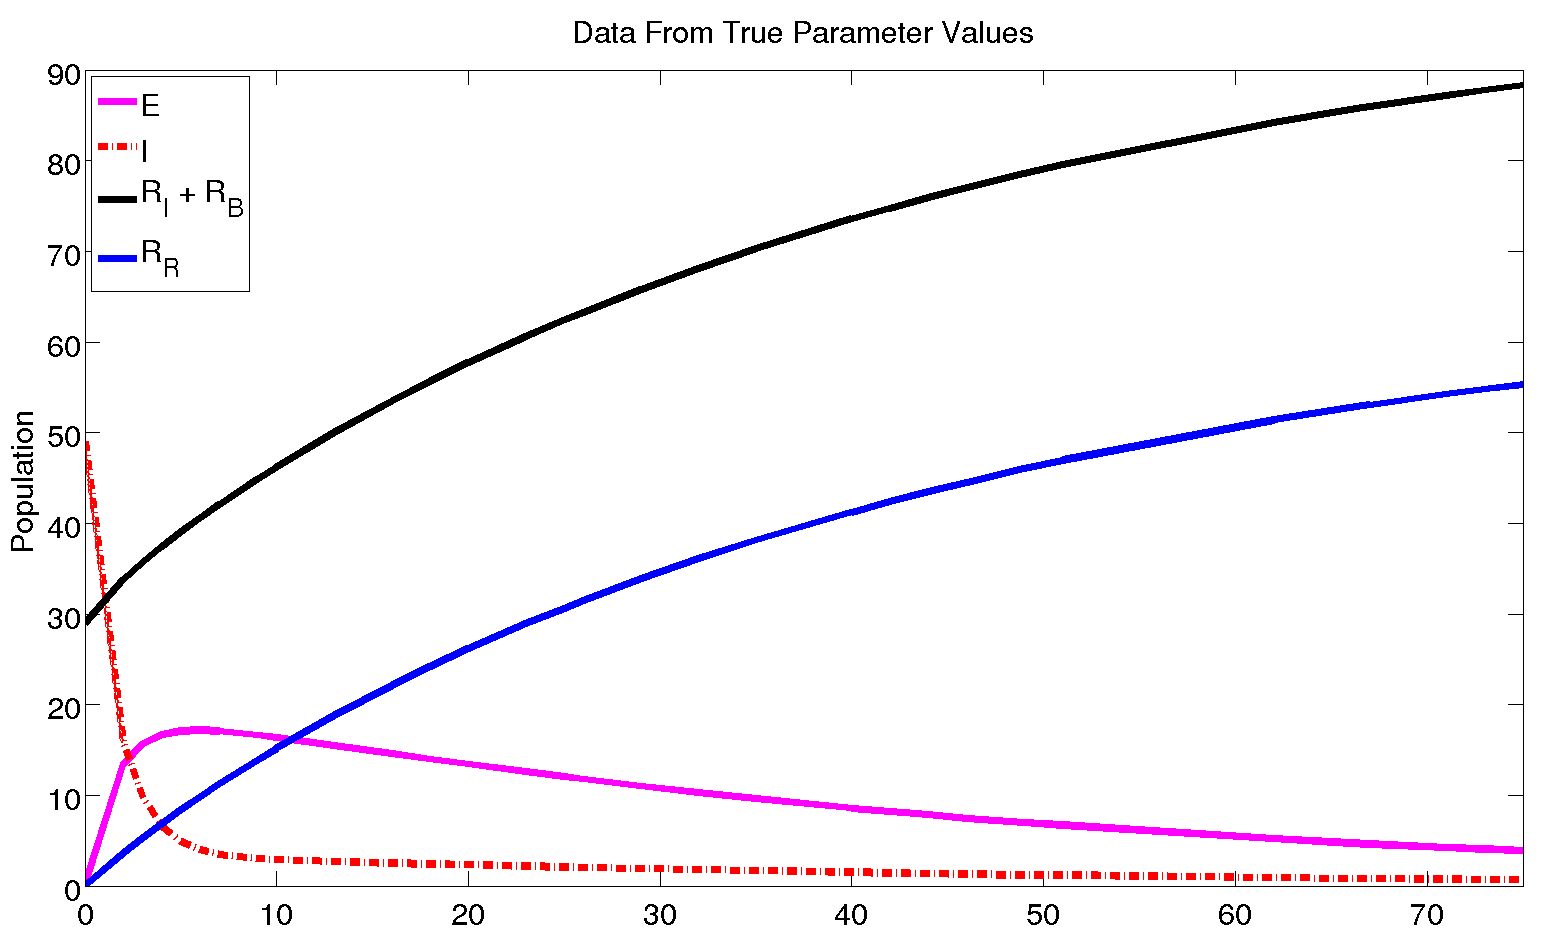
\includegraphics[scale=0.2]{model}
\end{frame}

\subsection{Sensitivity in the Inverse Problem}

\begin{frame}{Sensitivity in the Inverse Problem}
\centering
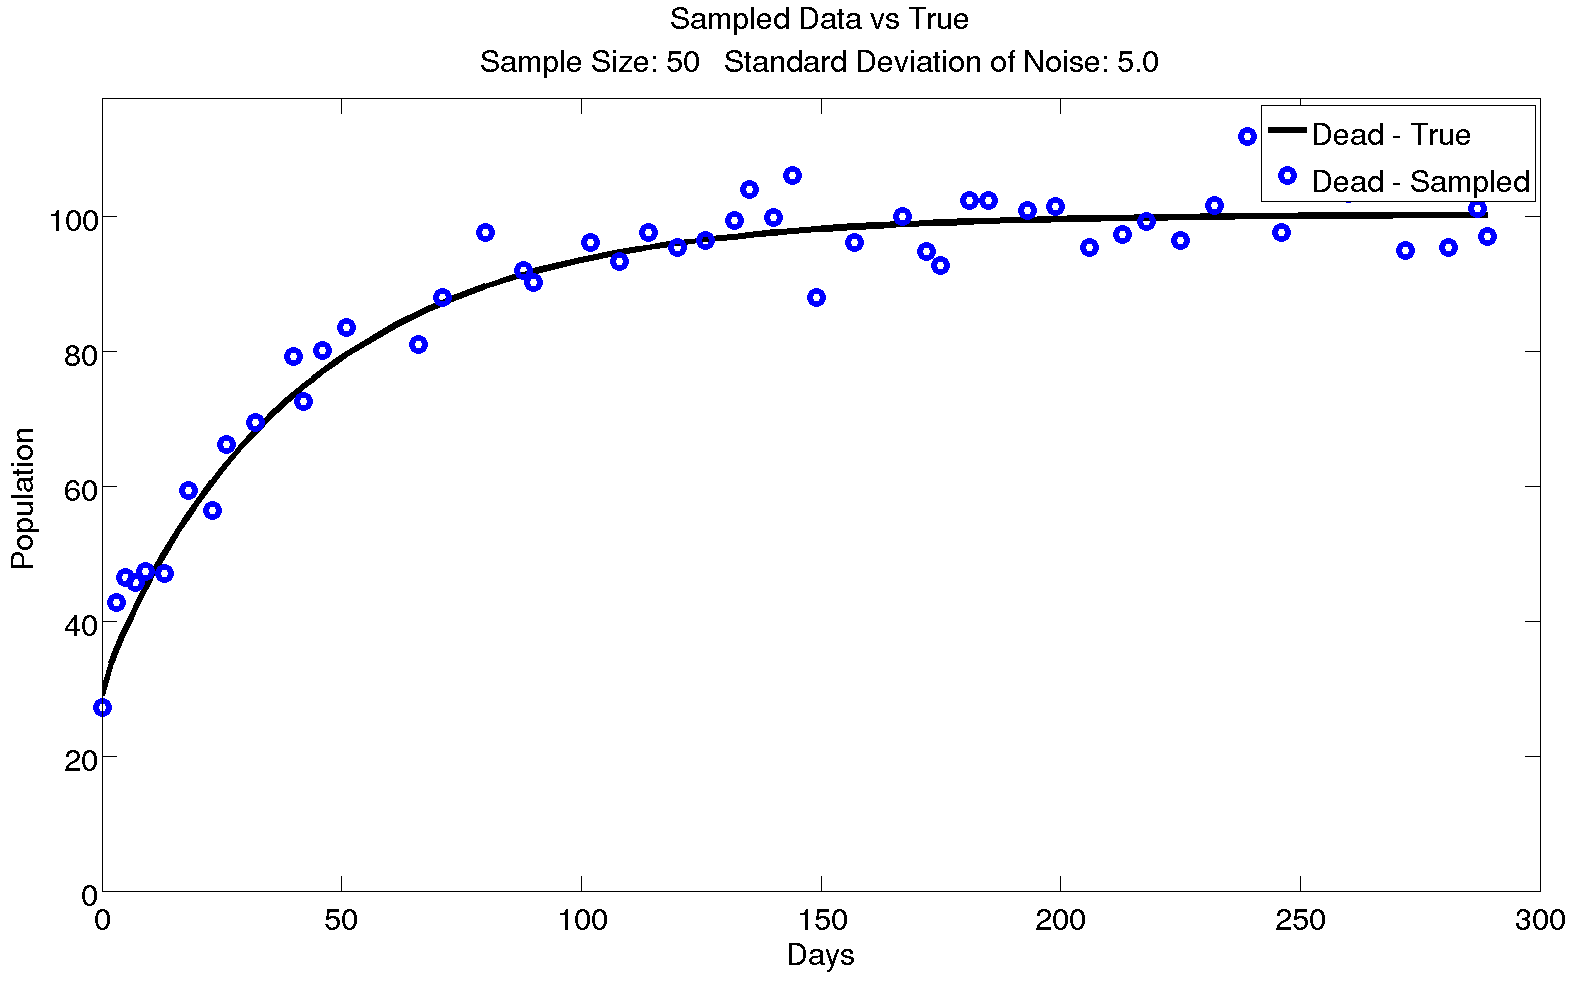
\includegraphics[scale=0.2]{noise}
\end{frame}

\subsection{MCMC}

\begin{frame}{MCMC}
\centering 
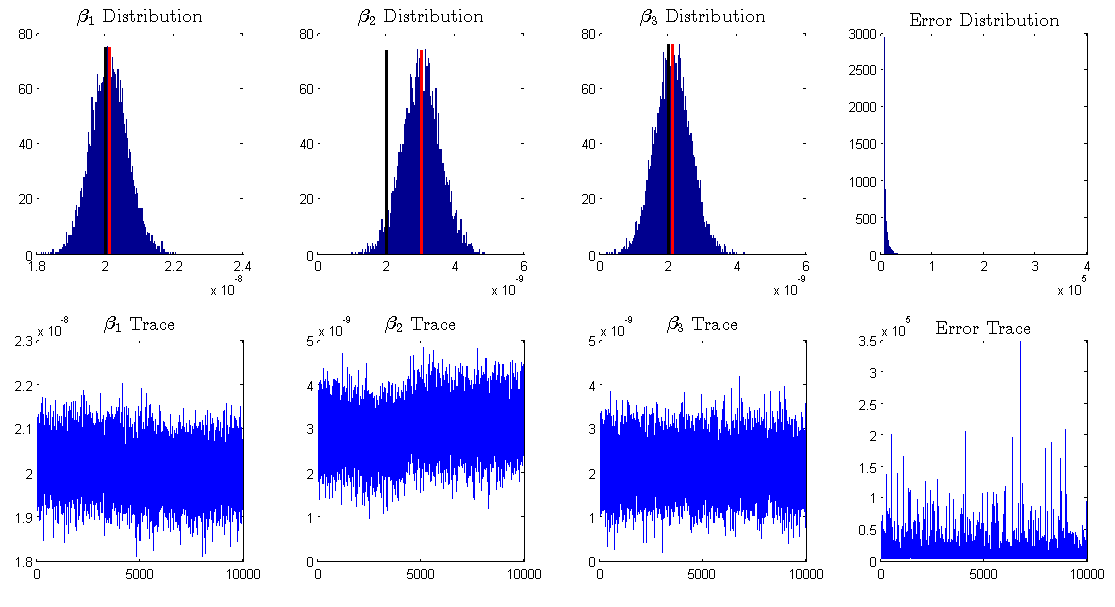
\includegraphics[width = 11.8cm]{mcmcoutput}
\end{frame}

\begin{frame}{Results}
\begin{table}[H]
\centering
\tiny
\noindent\makebox[\textwidth]{%
\begin{tabular}{rr|rrrrrr}
\hline
Sample Size & Noise $\sim N(0,s^2)$& $\bar{\beta_1}$ & $\bar{\beta_2}$ & $\bar{\beta_3}$ & $SD(\hat{\beta_1})$ & $SD(\hat{\beta_2})$ & $SD(\hat{\beta_3})$ \\
\hline
25 & 0 & 1.83e-8 & 5.49e-9 & 2.16e-9 & 4.98e-10 & 5.04e-10 & 4.97e-10 \\
50 & 0 & 1.99e-8 & 2.01e-9& 2.00e-9 & 5.17e-10 & 5.60e-10 & 4.99e-10 \\
25 & 5 & 2.00e-8 & 7.02e-9 & 1.82e-9 & 5.28e-10 & 6.16e-10 & 5.00e-10 \\
50 & 5 & 1.55e-8 & 4.40e-9 & 2.59e-9 & 5.01e-10 & 5.04e-10& 4.96e-10\\
25 & 10 & na & na & na & na & na & na \\
50 & 10 & 2.01e-8 & 2.99e-9 & 2.11e-9 & 5.077e-10 & 5.23e-10 & 5.01e-10 \\
\hline
\end{tabular}
}
\caption{\scriptsize Results of MCMC for different sample sizes and different random noise}
\label{tab:mcmctable}
\end{table}
\end{frame}

\begin{frame}
\Huge Questions?
\end{frame}

\begin{frame}{References}

\begin{thebibliography}{3}
\setbeamertemplate{bibliography item}[text]
\tiny
\bibitem{cdc} Center for Disease Control. \emph{Questions and Answers: Estimating the Future Number of Cases in the Ebola Epidemic}, 2015. 

\bibitem{dynamics}J. Lewnard et. al. \emph{Dynamics and Control of Ebola virus Transmission in Montserrado, Liberia: a mathematical modeling analysis} Department of Epidemiology of Microbial Diseases. Yale, 
CT. Dec 2014. ttt{http://www.cdc.gov/vhf/ebola/outbreaks/2014-west-africa/qa-mmwr-estimating-future-cases.html}

\bibitem{WorldBank} ``Population Growth (annual \%)." The World Bank. Web. 26 Mar. 2015. http://data.worldbank.org/indicator/SP.POP.GROW. 

\bibitem{CDC2} ``Signs and Symptoms." Centers for Disease Control and Prevention. N.p., n.d. Web. 27 Mar. 2015. http://www.cdc.gov/vhf/ebola/symptoms/index.html. 

\bibitem{epic} "Case Fatality Rate for Ebolavirus." Epidemic : Molecular Epidemiology and Evolution of Viral Pathogens. Web. 17 Apr. 2015. http://epidemic.bio.ed.ac.uk/ebolavirus-fatality-rate. 

\bibitem{betaTerm}Nielsen, Carrie F., Sarah Kidd, Ansumana Sillah, Edward Davis, and Jonathan Mermin. ``Improving Burial Practices and Cemetery Management During an Ebola Virus Disease Epidemic — Sierra Leone, 2014." Centers for Disease Control and Prevention. \emph{Centers for Disease Control and Prevention,} 16 Jan. 2015. Web. 26 Mar. 2015.

\bibitem{deathRate} Epatko, Larisa. ``70 percent Ebola death rate? Here’s how they calculate it." \emph{PBS News Hours.} N.p., 16 Oct. 2014. Web. 26 Mar. 2015. http://www.pbs.org/newshour/rundown/70-percent-ebola-death-rate-calculate/. 

\bibitem{fitting} Shaby, Ben. ``Fitting the SIR model to data`` \emph{Statistical and Applied Mathematical Sciences Institute Undergraduate Workshop.} 18 May, 2010.   http://www.samsi.info/sites/default/files/Shaby\_sir\_lab.pdf  
\bibitem{dataset} Rivers, Caitlin.  ``Consolidated, machine-readable ebola situation reports``\emph{Virgina Tech Network Dynamics and Simulation Science Laboratory.} 31 Dec, 2014. https://github.com/muxspace/ebola.sitrep 



\end{thebibliography}	

\end{frame}

\end{document}